\vspace{-15pt}
\section{Introduction}

\begin{figure*}[h]
    \centering
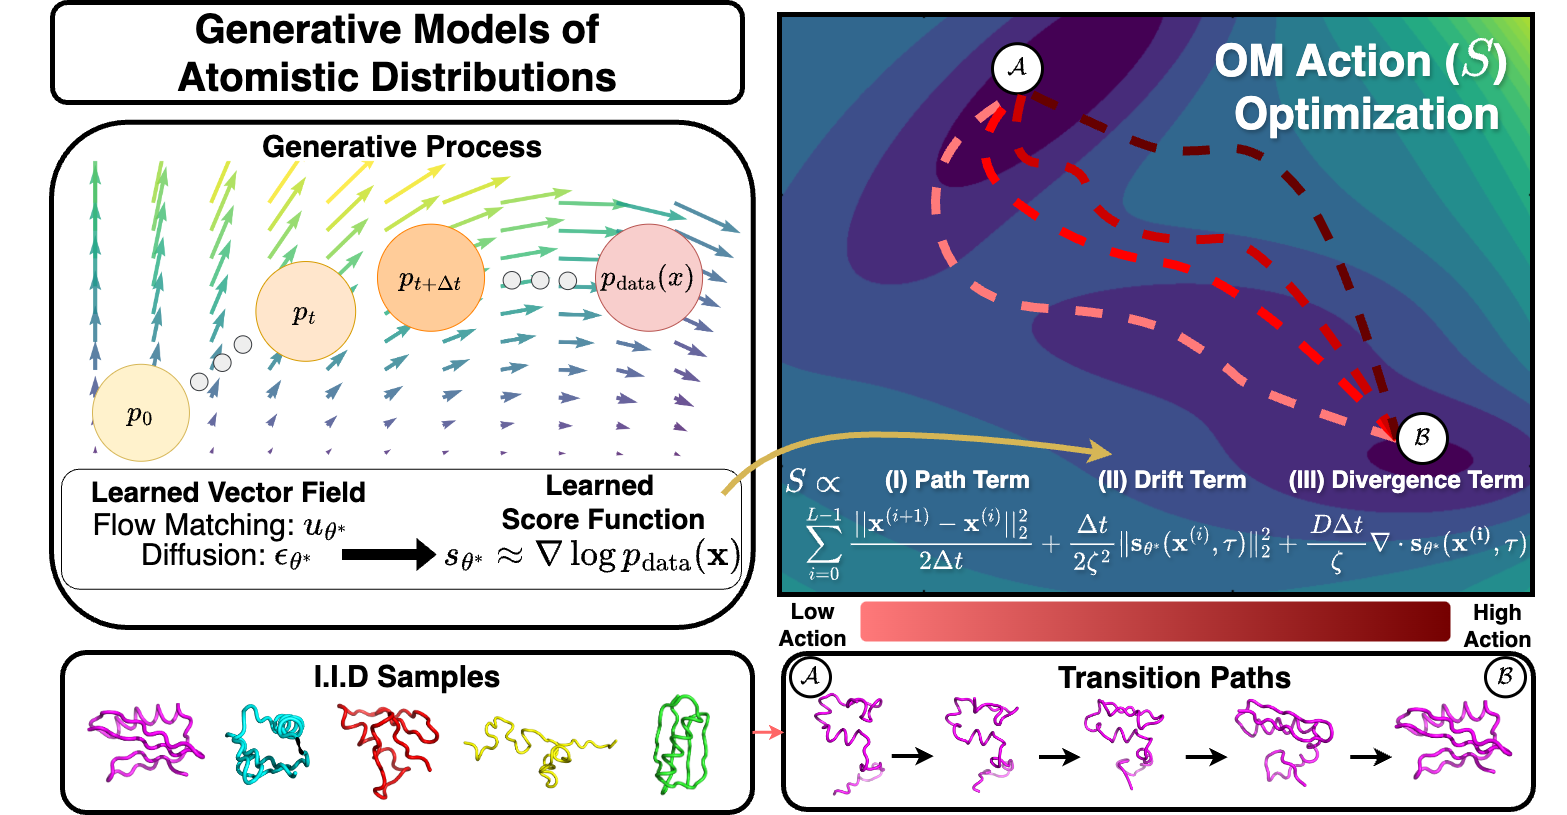
\includegraphics[width=\linewidth] {Figures/fig1.png}
    \caption{\textbf{Proposed Onsager-Machlup Action Optimization Schematic.} \textbf{(Left)} Atomistic generative models produce statistically independent samples via integration along a learned vector field, from which a score estimate, $s_{\theta^*} \approx \nabla \log  p_\text{data}(\xx)$, can be extracted. The score can be interpreted as a drift term in the stochastic dynamics induced by the generative model. \textbf{(Right)} This connection can be leveraged to repurpose atomistic generative models to find high-probability transition paths between samples on the data manifold by minimizing the OM action functional, \eqref{eq:generative_om_action}. The OM action has three terms which prioritize (I) low distance between adjacent points on the discretized path, (II) low-norm drifts, and (III) convexity of the underlying energy landscape. The variables are as follows: path point $i$ ($\xx^{(i)}$), trajectory length ($L$), timestep ($\Delta t$), friction ($\zeta$), diffusion ($D$), latent time ($\tau$). The underlying score $s_{\theta^*}$ remains frozen throughout OM optimization. Although valid for any data distribution, in the special case of Boltzmann-distributed data, our approach has the natural interpretation of transition path sampling on a potential energy surface with an atomistic force field.}
    \label{fig:mb_result}
    \vspace{-5pt}
\end{figure*}


Efficiently sampling the configurational distribution of high-dimensional molecular systems is a grand challenge in statistical mechanics and computational science \cite{tuckerman2023statistical, frenkel2023understanding}. A key area of interest is the sampling of rare, transition events between two stable configurations, such as in chemical reactions or protein folding \cite{bolhuis2002transition, dellago2002transition}. This task, broadly known as transition path sampling (TPS), is challenging due to the presence of energy barriers, which create a substantial difference in timescales between rare events and the fastest dynamical motions of the system (e.g., bond vibrations). This has inspired a rich line of literature on enhanced sampling techniques \cite{torrie1977nonphysical, swendsen1986replica, laio2002escaping, laio2008metadynamics, tiwary2013metadynamics, valsson2014variational}. More recently, machine learning (ML) based methods have gained popularity for accelerating TPS by learning a control drift term to bias a system towards a desired target state \cite{sipka2023differentiable, holdijk2024stochastic, du2024doob, seong2024transitionpathsamplingimproved}. However, these approaches rely on highly specialized training procedures and fail to exploit the growing quantity of atomistic simulation and structural data \cite{bank1971protein, vander2024atlas, lewis2024scalable}, and the increasing availability of high-quality atomistic conformational generative models \cite{abramson2024accurate, lewis2024scalable, jing2024alphafoldmeetsflowmatching, zheng2024predicting}. 

Generative models can produce unbiased, independent samples from atomistic conformational ensembles \cite{noe2019boltzmann, zheng2024predicting, jing2024alphafoldmeetsflowmatching} and have shown the potential to generalize across chemical space \cite{klein2024transferable, lewis2024scalable}. However, they have not been directly used for TPS due to the use of uncorrelated states during training. In this work, we propose a conceptually simple post-training method to repurpose generative models to perform TPS in a zero-shot manner. Our core idea exploits the fact that generative models based on denoising diffusion \cite{ho2020denoising} and flow matching \cite {lipman2022flow} induce a set of stochastic Langevin dynamics on the data manifold, governed by their learned \textit{score} function. Drawing inspiration from statistical mechanics, the probability of paths sampled from these dynamics can be characterized by a quantity known as the Onsager-Machlup (OM) action functional \cite{OMIbasic}. As a result, we can identify high-probability paths between arbitrary points on the data manifold directly from first principles by minimizing the OM action with gradient-based optimizers. In the specific case where the data are Boltzmann-distributed, the learned score approximates the underlying atomistic force field \cite{arts2023two}, and our approach has the direct, physical interpretation of TPS on a potential energy surface at a finite temperature.

Our approach has a number of key advantages:
\vspace{-5pt}
\begin{enumerate}
    \itemsep-1pt
    \item \textbf{Scalability:} We do not require any training procedure specific to TPS, and instead exploit pre-trained generative models. This makes our approach scalable as models and datasets continue to grow, and generalizable to new systems without retraining. 
    \item \textbf{Flexibility:} We can incorporate physical parameters such as the time horizon and temperature when sampling paths without modifying the underlying generative model.
    \item \textbf{Efficient Diversity:} We leverage the stochasticity of generative models to produce diverse candidate paths more efficiently than traditional methods.
\end{enumerate}
\vspace{-7 pt}
We validate our approach on systems of increasing complexity. Starting with the 2D Müller-Brown potential (Section \ref{sec:mb_results}), we build intuition and show accurate estimation of reaction rates and committor functions using our sampled transition paths. On alanine dipeptide (Section \ref{sec:alanine_dipeptide_results}), our method recovers accurate free energy barriers and outperforms metadynamics and shooting algorithms in efficiency. For fast-folding proteins (Section \ref{sec:fastfolders}), OM action minimization with diffusion or flow-matching models yields transition path ensembles closely aligned with reference MD at a fraction of the cost of traditional MD. Finally, we show that OM optimization with generative models trained on tetrapeptide configurations enables zero-shot TPS on new sequences (Section \ref{sec:tetrapeptides}). Overall, our work demonstrates the promise of repurposing pre-trained generative models as a general-purpose approach for transition path sampling.

% Finally, in Section \ref{sec:classical_ff}, we show that our OM framework can be used to quickly generate highly accurate, all-atom transition pathways for chignolin using a differentiable, classical force field.





